%%%%%%%%%%%%%%%%%%%%%%%%%%%%%%%%%%%%%%%%%
% Journal Article
% LaTeX Template
% Version 1.3 (9/9/13)
%
% This template has been downloaded from:
% http://www.LaTeXTemplates.com
%
% Original author:
% Frits Wenneker (http://www.howtotex.com)
%
% License:
% CC BY-NC-SA 3.0 (http://creativecommons.org/licenses/by-nc-sa/3.0/)
%
%%%%%%%%%%%%%%%%%%%%%%%%%%%%%%%%%%%%%%%%%

%----------------------------------------------------------------------------------------
%	PACKAGES AND OTHER DOCUMENT CONFIGURATIONS
%----------------------------------------------------------------------------------------

\documentclass[twoside]{article}

\usepackage{etex}
\usepackage{tikz} %graphics
\usepackage{tikz-qtree} % tree macros
\usepackage{tikz-dependency} % tree macros
\usepackage[sc]{mathpazo} % Use the Palatino font
\usepackage[T1]{fontenc} % Use 8-bit encoding that has 256 glyphs
\linespread{1.5} % Line spacing - Palatino needs more space between lines
\usepackage{microtype} % Slightly tweak font spacing for aesthetics
\usepackage{listings}

\usepackage[hmarginratio=1:1,top=32mm,columnsep=20pt]{geometry} % Document margins
\usepackage{multicol} % Used for the two-column layout of the document
\usepackage[hang, small,labelfont=bf,up,textfont=it,up]{caption} % Custom captions under/above floats in tables or figures
\usepackage{booktabs} % Horizontal rules in tables
\usepackage{float} % Required for tables and figures in the multi-column environment - they need to be placed in specific locations with the [H] (e.g. \begin{table}[H])
\usepackage{hyperref} % For hyperlinks in the PDF

\usepackage{lettrine} % The lettrine is the first enlarged letter at the beginning of the text
\usepackage{paralist} % Used for the compactitem environment which makes bullet points with less space between them

\usepackage{abstract} % Allows abstract customization
\renewcommand{\abstractnamefont}{\normalfont\bfseries} % Set the "Abstract" text to bold
\renewcommand{\abstracttextfont}{\normalfont\small\itshape} % Set the abstract itself to small italic text

\usepackage{titlesec} % Allows customization of titles
\renewcommand\thesection{\Roman{section}} % Roman numerals for the sections
\renewcommand\thesubsection{\Roman{subsection}} % Roman numerals for subsections
\titleformat{\section}[block]{\large\scshape\centering}{\thesection.}{1em}{} % Change the look of the section titles
\titleformat{\subsection}[block]{\large}{\thesubsection.}{1em}{} % Change the look of the section titles

\usepackage{fancyhdr} % Headers and footers
\pagestyle{fancy} % All pages have headers and footers
\fancyhead{} % Blank out the default header
\fancyfoot{} % Blank out the default footer
\fancyhead[C]{Dependency-Based QA $\bullet$ 2015 $\bullet$ CMPSCI 585} % Custom header text
\fancyfoot[RO,LE]{\thepage} % Custom footer text

\usepackage{caption}
\usepackage{amsmath}
\usepackage{stmaryrd}

% ----------------

% Default fixed font does not support bold face
\DeclareFixedFont{\ttb}{T1}{txtt}{bx}{n}{12} % for bold
\DeclareFixedFont{\ttm}{T1}{txtt}{m}{n}{12}  % for normal

% Custom colors
\definecolor{deepblue}{rgb}{0,0,0.5}
\definecolor{deepred}{rgb}{0.6,0,0}
\definecolor{deepgreen}{rgb}{0,0.5,0}

% Python style for highlighting
\lstset{
language=Python,
basicstyle=\ttm,
otherkeywords={self},             % Add keywords here
keywordstyle=\ttb\color{deepblue},
emph={MyClass,__init__},          % Custom highlighting
emphstyle=\ttb\color{deepred},    % Custom highlighting style
stringstyle=\color{deepgreen},
frame=single,                     % Any extra options here
showstringspaces=false,           % 
breaklines=true,
postbreak=\raisebox{0ex}[0ex][0ex]{\ensuremath{\color{red}\hookrightarrow\space}},
}

%----------------------------------------------------------------------------------------
%	TITLE SECTION
%----------------------------------------------------------------------------------------

\title{\vspace{-5mm}\fontsize{18pt}{12pt}\selectfont\textbf{Dependency-Based Structures\\For Question Answering}} % Article title

\author{
\large
\textsc{Alan J. Zaffetti}\\[2mm]%\thanks{A thank you or further information}\\[2mm] % Your name
\normalsize University of Massachusetts Amherst \\ % Your institution
\normalsize \href{mailto:azaffett@umass.edu}{azaffett@umass.edu} % Your email address
%\vspace{-5mm}
}
\date{}

%----------------------------------------------------------------------------------------

\begin{document}

\maketitle % Insert title

\thispagestyle{fancy} % All pages have headers and footers

%----------------------------------------------------------------------------------------
%	ABSTRACT
%----------------------------------------------------------------------------------------

\begin{abstract}

\noindent Question answering (QA) is a notoriously difficult task, requiring massive human effort, and usually resulting in complex systems.  I introduce parsed dependency graphs to represent NL setences and develop a baseline rule-based technique for answering forms of factual-questions.  Finally, I apply my method to a portion of the academic Wikipedia dataset (Carnegie Mellon, University of Pittsburgh).  I achieve 10\% accuracy for factual-questions in the instruments section, and 5\% over all questions in that category. 

\end{abstract}

%----------------------------------------------------------------------------------------
%	ARTICLE CONTENTS
%----------------------------------------------------------------------------------------

\section{Introduction}

\subsection{Motivation}

\lettrine[nindent=0em,lines=3]{T}he problem of question answering is a hard one because it is composed of multiple steps all of which are imperfect, and introduce error.  It is saved only by the fact that it is modular; tasks can be broken up into smaller and less complicated subtasks.  In a question answering system, this includes the methods used to break text up into sentences or sometimes individual tokens (\textit{tokenizer}); a technique for parsing sentences into a structured form (\textit{parser}); a strategy for representing structured facts derived from these parses (\textit{knowledge representation}); and finally a way to query the representation (\textit{IR}). Of course, there are more subprocesses within these.

The modularity of a system is nice for two reasons.  (1) it reduces the complexity of the system as a whole; and (2) it makes each step accountable for its performance on the system.  You may not trust the modules individually, but are more apt to trust the system as a whole because you can always find a \textit{better} tokenizer, or a \textit{faster} parser.  The modules on my system have their limitations.  For instance, my parser module does not handle unicode, and my tokenizer is brittle, but they can always be subbed out for other, better systems.

\subsection{Overview}

My system hopes to accomplish baseline fact-based \textit{wh}-QA (i.e. mostly \textit{what}, but perhaps \textit{when}, \textit{where}, etc.), while providing a framework for effecient QA methods at scale. However, this paper does not describe an end-to-end system, nor is the final project meant to accomplish this goal.  Instead, I will focus on demonstrating how my system ingests parsed sentences into dependency graph structures; then, finally show how QA can be done.  While I only focus on fact questions in this paper, the \textit{Discussion} section will comment on how to extend the QA to other types of question classes and domain.

I am using an academic Wikipeida dataset (Carnegie Mellon, University of Pittsburgh) for most of my tests.  For the others, I use hand constructed tests.  The corpus consists of question-answer pairs and links to the text document containing an answer.  The questions are subdivided by topic and difficulty (and this is clearly marked for each example). The dataset will be discussed in more detail in the \textit{Dataset} section below.

\subsection{Background}

\subsection{Overview}

Question answering (QA) is a discipline within computer science, information retrieval (IR), and natural language processing (NLP) focused on building systems capable of answering questions posed in natural language. A QA implementation typically queries a structured database of knoweldge, or set of unstructured documents.  Systems attempt to deal gracefully with the wide range of question types such as: \textit{fact}, \textit{list}, \textit{definition}, \textit{how}, \textit{why}, \textit{hypothetical}, \textit{semantically constrained}, or \textit{cross-lingual questions}.

\subsubsection{Dependency Parser}

The dependency parsing turns sentences into a structed form.  A dependency parser can work as a stand alone tool, or a constituency tree conversion tool.  In this case a constituency conversion tool, Stanford Dependencies (freely available online \footnote{https://github.com/dmcc/PyStanfordDependencies}), was used.  Standard trees were generated using Stanford CoreNLP and converted using a trained model.  Since this paper is not about the process of creating dependencies we will not go over the technical details of how this is done.

A dependency parse orders words in a DAG structure, such that commanding words (e.g. heads) are above their dependents (e.g. non-heads).  This can be formalized by a series of head-structure rules which is an augmentation of a CFG, also giving information about which productions are non-head and which one is a head.  Models might be trained by learning these rules and labelled examples.  Labelled arrows, then, replace trees when going from a standard constituency parse to a dependency structure.

The resulting parse yields a formalism of a system of 42 universal dependency relations \footnote{http://universaldependencies.github.io/docs/u/dep/} which include nominal subjects, passive nominal subjects, compound noun phrases, adjectival modifiers, numeric modifiers, and many more.  These define relations over individual words in the parse.  Relations connect words on a syntactic level, but meaningful semantics is not hard to derive from these trees.  For example, given a parse of the sentence ``The boy fished the tank'', we can easily read from the parse who is the dooer of the action \textit{boy} (a.k.a. the agent), and who is a patient, in this case \textit{tank}.  Figure \ref{fig:deps} shows what this looks like.

\begin{figure}
\centering
\caption{In the sentence, dependency relations cover all words in the parse, embedding syntactic relationships, which have a semantic reading.  In this example, \textit{boy} is the nominal subject (\textit{nsubj}) of the root (\textit{fish}) and the direct object (\textit{dobj}) is \textit{tank}.} \label{fig:deps}
\begin{dependency}[edge horizontal padding=10pt]\begin{deptext}[column sep=0.3cm]ROOT \& DT \& NN \& VBD \& NNS \& .\\ROOT \& The \& boy \& fished \& tanks \& .\\\end{deptext}\depedge{3}{2}{det}\depedge{4}{3}{nsubj}\depedge{4}{5}{dobj}\depedge{4}{6}{punct}\depedge{1}{4}{root}\end{dependency}
\end{figure}

This is the basis of the representation of the question answering system.  By relating objects through the dependency structure, we are able to extract key information about the facts that the sentence relays.

\paragraph{Projective v. Non-projective Dependencies} Projective dependencies are used to better represent free word order in dependency structure; there are also a number of other differences in the phrase structure.  My system uses non-projective dependencies as these offer good results for most constructions of English.

\section{Related Work}

\subsection{Systems}

Most successful examples of question answering systems have closed-domains.  These systems become expert savants on a single topic (e.g. medicine, baseball, etc.).  They ingest documents, learn structured databases, and ontologies which define all of the words in the target domain.  Other closed-domain systems restrict the types of questions which may be asked.  A prominent intersection between these categories are intelligent smart phone assistants such as \textit{Siri}, or \textit{Ok, Google}.  In contrast, open-domain QA can deal with any subject or possible type of question.  For such a system to be successful, it must ingest many documents from many distinct sources. A prominent example of such a system was IBM's Jeoparody!-playing computer \textit{Watson}, and even this was extremely complicated, and took years of engineering.  \textit{Watson} is currently being applied to medical informatics domains, where it has more practical uses.


\subsection{Research}

The history of question answering research efforts have used a number of techniques, including rule based systems (Riloff, et. al., 2000 \cite{ril00}), machine-translation (Bao, et. al., 2014 \cite{bao14}), or hybrids (Pakray, et. al., 2014 \cite{pak11}). However, lately dependency parses have dominated many question answering tasks.  Knowledge based systems exist (Hermjakob, et. al., \cite{her02}, and information retrieval is also a relative facet of study since many systems including this one use it as their main modus operandi (i.e. searching semi-structured documents).

\subsubsection{Dependency N-grams}

One could gain lots of information on sentence struture by making $N$-grams over dependency graph spines.  This has proven successful even when $N$-grams do not include dependency relations.  This is due to the fact that dependency relations represent the longer-distance relationships between words in a sentence, where more traditional phrasal constituents combine nearby words to create a phrase.

This kind of relational technique has proved successful in tasks such as surface realization (language generation task), where dependency-based $N$-grams proved more helpful than constituents in representing accurate syntax (Guo, et. al., 2008) \cite{guo08}.  A system which simply counts instances of $N$-grams could be used to gain insight into what types of relationships are possible.

Although, I do not pursue this method in this paper, I bring up the practice of $N$-gram semantics because it is a useful technique.  However, using the $N$-gram formalism does have its drawbacks (including loss of information about dependency relations).

\section{Dataset}

\subsection{Overview}

The dataset is an academic QA corpus from 2010\footnote{These data were collected by Noah Smith, Michael Heilman, Rebecca Hwa, Shay Cohen, Kevin Gimpel, and many students at Carnegie Mellon University and the University of Pittsburgh between 2008 and 2010. This research project was supported by NSF IIS-0713265 (to Smith), an NSF Graduate Research Fellowship (to Heilman), NSF IIS-0712810 and IIS-0745914 (to Hwa), and Institute of Education Sciences, U.S. Department of Education R305B040063 (to Carnegie Mellon).}.  It contains curated, and cleaned text-only versions of a variety of Wikipedia pages as an underlying dataset.  It also contains labelled question data separated by topic, paired with the question's answer, and which dataset file contains the answer.  Questions are also rated by difficulty, once by the creators of the question, and again by the one's who've answered them.  Many questions are repeated twice to allow training on multiple correct responses.  Topics are broken up into sets, each having its own distinct theme.

\definecolor{auburn}{rgb}{0.43, 0.21, 0.1}
\definecolor{applegreen}{rgb}{0.55, 0.71, 0.0}
\definecolor{americanrose}{rgb}{1.0, 0.01, 0.24}
\definecolor{azure}{rgb}{0.0, 0.5, 1.0}

\begin{figure}
\caption{The topics in the complete dataset.  For this assignment, I narrowed down the domain to only the Musical Instruments section. \label{fig:datastat}}
\begin{tabular}{|l|l|p{11.5cm}|}
\hline
\multicolumn{3}{|c|}{Academic QA Dataset Statistics} \\
QA Pairs & 1459 & \\ \hline
Sets & 6 & {\color{applegreen}Animals}, {\color{azure}Musical Instruments}, {\color{auburn}Cities}, {\color{americanrose}Famous scientists}, {\color{orange}Languages}, {\color{black}Famous artists}\\ \hline
Topics & 60 & {\color{applegreen}Ant, Octopus, Cougar, Koala, Giant Panda, Lobster, Butterfly, Dragonfly, Eel, Zebra}, {\color{azure}Piano, Lyre, Violin, Trumpet, Drum, Flute, Cymbal, Guitar, Xylophone, Cello,} {\color{auburn}Berlin, Saint Petersburg, Melbourne, Kuala Lumpur, Antwerp, Jakarta, Taipei, Montreal, San Francisco, Nairobi,} {\color{americanrose}Newton, Volta, Watt, Tesla, Pascal, Celsius, de Coulomb, Faraday,  Avogadro, Becquerel}, {\color{orange}Portuguese, Vietnamese, Malay, Arabic, Swahili, Finnish, Korean, Chinese, Turkish, Swedish,} {\color{black}Picasso, Klimt, Michelangelo, da Vinci, Rockwell, Renoir, Mondrian, van Gogh, El Greco, Pollock} \\ \hline
\end{tabular}
\end{figure}

\begin{figure}
\centering
\caption{Frequency of the most common 40 question types in the corpus. \label{fig:qtypes}}
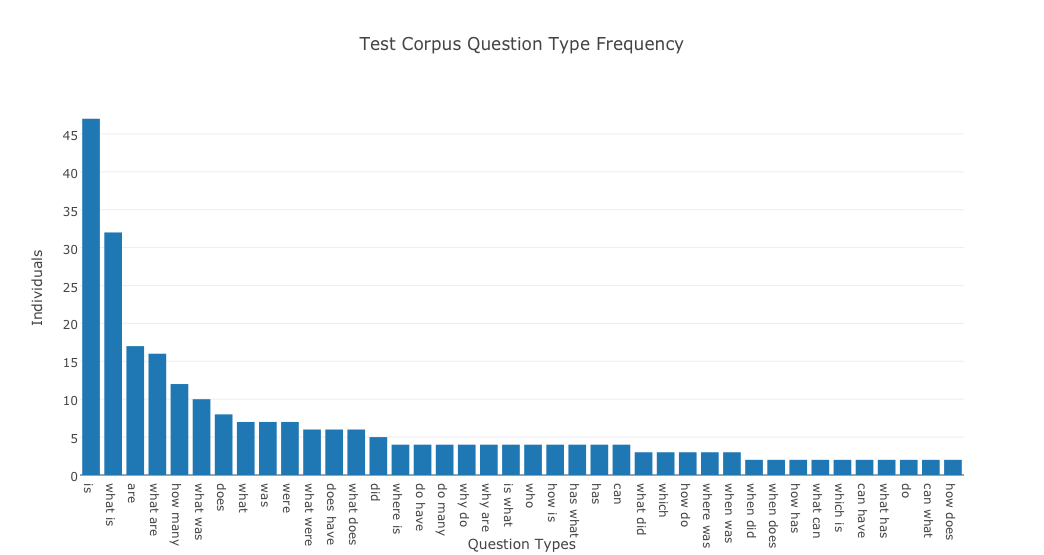
\includegraphics[width=400px]{figures/qtypes-test.png}
\end{figure}

Table \ref{fig:datastat} shows an example of the question style in the corpus.

\subsection{Preparation of Data}

Data was compiled from the corpus and a choice was made to narrow the domain to musical instruments only.  This was a practical choice, as the number of questions in the original corpus was quite large $(N=1459)$ and a smaller domain would still accomplish the primary goal of having a variety of question types.  Using scripts available in the code, I prepared the unstructured text into JSON files, effectively splitting off each individual subtopic into its own document.  I repeated this for the wiki pages and for the question answer pairs (all available in the \texttt{data/} section of the repository.  The final corpus has 10 topics and 280 unique questions spanning a range of question types.

\section{Method}

\subsection{Overview}

Using parsed JSON dependencies produced from the corpus data, it is now possible to begin QA.  The basic strategy of my method was to learn as much as possible from the set of question answer pairs.  This includes partititioning them into a large number of question types (question words such as `that`, `which`, `what`, but also `how many` etc.).  Secondly, using the dependency parses from these, I can gain information from parses for both the question and answer.  For the question I show how I extract a "selector" (query), which I use to search the data in the IR step.  For the answer parse, I determine what dependency relation contains reference to the correct answer in the parse.  That is, in a standard factual phrase or sentence, what part of that sentence contains the answer we are looking for?

\subsection{Question Types}

I use the following regular expression

\begin{equation} \label{eq:qre}
\begin{split}
\text{\textbackslash b(who|what|where|why|when|which|how|many|can|}\\
\text{is|are|do|does|did|were|was|will|has|have|had)\textbackslash b}
\end{split}
\end{equation}

To find all question and tense words (including \textit{many}) in a question.  It's imperfect but it works fairly well at making a rough question class clustering.  I limit the results to find two such question and tense words for each question type.  This expression yields dozens of question types, the top 40 of which are displayed in Figure \ref{fig:qtypes} and Figure \ref{fig:whatqs}.

\subsubsection{Algorithm}

\begin{figure}
\caption{Full question type categories are generated in this way.  The regular expression in Figure \ref{eq:qre} is also used but in other aspects of generation, such as in question parsing. \label{fig:alg1}}
\lstinputlisting{algorithms/get-question-types.py}
\end{figure}

\subsection{Selectors}

Selectors are generated from the data using rules that differ for each question type.  The selectors are "learned" from the question answer pair data in the sense that the rules are extracted and then ordered by frequency.  This creates a "cascading" rule-based system in which the most likely (highest weighted) rule is tried first, then the next, until one rule is finally matched.  When a rule is matched this is made the "selector" for the sentence (i.e. the unique query terms used to find references to the topic in natural context).  The selector itself (not including question type) is made up of three parts, the `agent,' the `theme,' and the `patient.'

\subsubsection{Agent}

The agent (or referent) is the part of the answer that contains the reference to the subject.  For questions depending on the topic, (e.g. violin, Avagadro) it could be the actual word, its plural or a pronoun (e.g. `it', `he').  In general, this is the subject of the sentence, although one must be careful about passives (handled with \texttt{nsubjpass}).  It is selected by first finding reference to the the topic, and if none exists, the subject of the sentence is chosen, as described above.

\subsubsection{Theme}

The theme (or root) is simply the root of the dependency tree.  The dependency tree naturally aligns the purpose of the sentence at the root of the tree, so this information is very useful when filtering through the corpus.  However there are some instances (such as when the root of the sentence is a question word) that we do not have a theme.

\subsubsection{Patient}

The patient is the object of the sentence.  It is selected after the agent so that it does not accidentally collide with the selected agent.  There are many cases where a patient does not exist (such as instances of `what' questions) where we set the patient term to None.

\subsubsection{Algorithm}

\begin{figure}
\caption{This is the overall algorithm for getting distributional information about the selectors.  The step which actually sums up the values is omitted, but in implementation, it would map the question type to the three selector components. \label{fig:alg2}}
\lstinputlisting{algorithms/learn-selectors.py}
\end{figure}

\begin{figure}
\caption{Examples of \textit{what} questions \label{fig:whatqs}}
\begin{tabular}{|l|l|l|}
\hline
what is the most common color of ants? & what happened in 1894? \\ \hline
what family is the panda a part of? & what religion holds majority in melbourne? \\ \hline
what is coulomb's law? & what led pascal to his religious conversion? \\ \hline
what is panda diplomacy? & what happened in 1810? \\ \hline
what's the population of kuala lumpur? & what happened in 1894? \\ \hline
\end{tabular}
\end{figure}

\subsection{IR Step}

The most important step of the algorithm is Information Retrieval.  This is the part where the selectors do their work to match results in the actual corpus.  Emprical results are provided across various question types, but not for all question types, primarily because selector rules failed to fire for many question types (see Figure \ref{fig:result1}).  Secondly, it seems that many selector rules still fail to capture the full syntactic variation present in the real Wiki texts.

\subsubsection{Special Treatment of Tense Questions}

Tense questions are those which lack question words (`which,' `what,' `who,' etc.), having only tense words (`is,' `are,' etc.)  These are thresholded, so that if a result is found, it returns \texttt{true} and \texttt{false} otherwise.  Negations are not handled natively, unless the negations come up explicitly in the corpus.

%------------------------------------------------

\section{Results}

\subsection{Overview}

I evaluated my results empirically to determine first, the quality and viability of the chosen selectors.  Then, I evaluated the actual IR step, how these selectors apply to the data to find answers.  The results for the selector step are displayed in Figure \ref{fig:result1}.  They represent an average $(p=.46)$ for accurate selector choice, some categories even reaching perfect accuracy, some in the middle, and a few at 0.  Obviously, those question types which did not make the selector step had very slim chance of actually firing during IR (which I verified).  In the end I saw results for the highest factual questions at 10\%.  The average for all question types was 5\%.

\begin{figure}[hb]
\centering
\caption{This graph evaluates the selectors found for each question type.  These were evaluated empirically to determine whether the query could ever possibly return results in the IR step.  This was easy to determine because sometimes (roughly half) the questions were incorrectly evaluated due to an inability to cover all question types.  In any case, the results as they stand, show that the selector generation algorithm worked best on `are,' `how many,' and `where is' questions.
\label{fig:result1}}
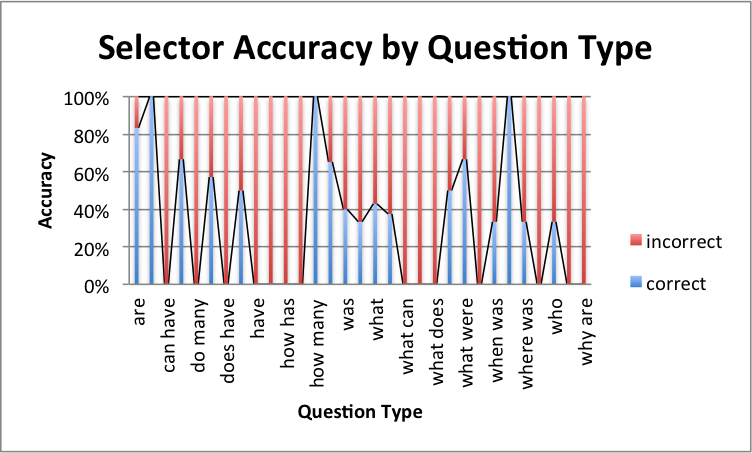
\includegraphics[width=400px]{figures/selector-accuracy.png}
\end{figure}

\section{Discussion}

\subsection{IR Limitations}

Not all questions or answers are created equal.  In natural language one can phrase things in an infinitude of different ways.  In syntactic structure alone, many variations of the above question and answer forms may be used, all refering to the same information. Morphologically, the evaluation is even more bleak; synonyms for words abound, and if no way to deal with these exist, one cannot possibly hope for a system to handle any of them.  So these two issues limit the ability of this mapping, where, although there may exist a singular semantic concepts for both question and answer, there is an infinitude of extensions of these, in practice.  Another problem is coreference, which is not handled in this system.

\subsection{Future Work}

This paper made an attempt at answering factual $wh$-questions using the corpus and constructed QA pairs.  Clearly, I have not come near to real QA in this paper;  this would have been an unreasonable goal.  Here are some items still reserved for future goals:

\paragraph{Inference} How to make logical inferences?
\paragraph{Learn Better} How to improve the learning step using structured probability models and machine learning?

%----------------------------------------------------------------------------------------
%	REFERENCE LIST
%----------------------------------------------------------------------------------------

%\begin{multicols}{2}
\begin{thebibliography}{9} % Bibliography - this is intentionally simple in this template

\bibitem{guo08}
Yuqing Guo, Josef van Genabith, Haifeng Wang (2008)
\newblock Dependency-Based N-Gram Models for
General Purpose Sentence Realisation

\bibitem{bao14}
Junwei Bao, Nan Duan, Ming Zhou, Tiejun Zhao (2014)
\newblock Knowledge-Based Question Answering as Machine Translation; \textit{Microsoft Research}
 
\bibitem{ril00}
Ellen Riloff and Michael Thelen  (2000)
\newblock A Rule-based Question Answering System for Reading Comprehension Tests

\bibitem{pak11}
Partha Pakray, Pinaki Bhaskar, Somnath Banerjee, Bidhan Chandra Pal, Sivaji Bandyopadhyay, Alexander Gelbukh (2011)
\newblock A Hybrid Question Answering System based on Information Retrieval and Answer Validation

\bibitem{her02}
Ulf Hermjakob, Eduard H. Hovy, and Chin-Yew Lin (2002)
\newblock Knowledge-Based Question Answering; \textit{Microsoft Research}

\end{thebibliography}
%\end{multicols}

%----------------------------------------------------------------------------------------

\end{document}
